\documentclass[12pt]{article}
\usepackage[utf8]{inputenc}
\usepackage[T1]{fontenc}
\usepackage[brazil]{babel}
\usepackage{indentfirst}
\usepackage{multicol}
\usepackage{graphicx}
\usepackage{multirow}
\usepackage[a4paper, top = 2.5cm, bottom = 2.5cm, footskip = 1cm]{geometry}
\usepackage{vwcol}
\usepackage{subfigure}
\renewcommand{\familydefault}{\sfdefault}
% necessário para ter várias seções dentro de seções
\setcounter{secnumdepth}{5}
\setcounter{tocdepth}{5}

\title{Manual do Bixo 2017}
\author{Centro Acadêmico Pata do Bisão, Gestão 2016/2}
\date{\today}

\begin{document}
%%% CAPA %%%
\begin{figure}
    \hspace*{-3.7cm}
\includegraphics{./imagem/capa2017.pdf}
\end{figure}
\thispagestyle{empty}

\clearpage
\begin{center}
  Este projeto está licenciado em Attribution-ShareAlike 4.0 International da Creative Commons. Para saber mais sobre a licença, você pode visitar este website: \texttt{https://creativecommons.org/licenses/by-sa/4.0/}
~\\[\baselineskip]
  \begin{figure}[h]
    \centering
    \begin{subfigure}
      \centering
      
\includegraphics[width=0.2\textwidth]{./imagem/cc_logo.pdf}
    \end{subfigure}
    \begin{subfigure}
      \centering
      
\includegraphics[width=0.2\textwidth]{./imagem/by_sa.pdf}
    \end{subfigure}
  \end{figure}
~\\[\baselineskip]

  O código fonte deste manual se encontra no repositório do Centro Acadêmico Pata do Bisão, você pode visitar neste website: \url{https://github.com/caccs/Manual-do-Bixo}.


  \vfill Copyright © 2013-\the\year \thinspace Centro Acadêmico Pata do Bisão
\end{center}

\thispagestyle{empty}

\clearpage
\setcounter{page}{1}

%%% ÍNDICE %%%
\clearpage
\tableofcontents

%%% SOBRE %%%
\clearpage
\section{SOBRE ESTE MANUAL}
Este manual foi baseado em um manual dos bixos existente do Centro Acadêmico de 2013, sendo ele aprimorado pelos CA da gestão de 2015/2 e também pela Atlética Raça Brisão. Na gestão 2016/2, foram adicionados ainda mais itens e seções, na expectativa de torná-lo cada vez mais completo. E agora na gestão 2017/2, adaptamos o manual para a nova grade a fim de podermos informá-los da melhor forma possível.

Esperamos que este manual te ajude de alguma forma sua nova vida acadêmica, calouro(a); caso você acredite que faltou algum item ou necessita de mais detalhes sobre determinado assunto, responda o formulário e conte para gente. :)

Caso precise urgentemente de alguma informação que não esteja aqui, pode nos contactar pela página do Facebook: \texttt{https://www.facebook.com/CACCS.UFSCar/}

Por fim, gostaríamos de agradecer ao Departamento de Computação por incentivar o Centro Acadêmico em todas as atividades que propomos, incluindo o Manual do Bixo. Vocês são 10/10. <3

\begin{flushright}
  Obrigado(a)!

  C.A. Pata do Bisão Gestão 2017/2
\end{flushright}


%%% BEM-VINDO %%%
\clearpage
\section{BEM-VINDO(a)!}
\noindent{\textbf{Olá, calouro(a) computeiro(a)!}}

Nós, alunos e docentes do Curso de Ciência da Computação de Sorocaba, lhe parabenizamos por ter vencido mais esta etapa em sua vida. Como você já deve saber, acabou de entrar numa das melhores universidades do país para cursar Ciência da Computação. 

Desejamos toda a força do mundo para seguir em frente e ir até o fim nessa jornada.

Gostaríamos de dizer que estamos disponíveis para dar qualquer apoio, seja no sentido acadêmico ou pessoal.

Saiba que é seu direito não querer participar de qualquer trote, mas saiba também que não custa nada entrar na brincadeira, desde que não passe dos limites. Afinal, você passou, véi, é federal! Sinta-se em casa e encontre nos veteranos grandes companheiros, porque, no fim, unidos somos mais fortes.


%%% BREVE INTRODUÇÃO AO CURSO %%%
\section{BREVE INTRODUÇÃO AO CURSO}
Independente de sua cidade natal, de estar morando sozinho, com os pais ou até em uma república, nós sabemos o quão diferente é a vida acadêmica do colégio e do cursinho. Sempre é uma grande mudança e um grande passo para qualquer jovem. Aqui nós damos algumas dicas sobre as matérias dos seus primeiros semestres e como funciona o sistema de requisitos de nosso curso.

Na UFSCar utilizamos o sistema de créditos - você pode entender créditos como horas semanais de um semestre - em que, no curso Ciência da Computação você precisará de 217 créditos para se formar sendo eles: 109 de disciplinas obrigatórias, 56 de optativas, 24 do Trabalho de Graduação ou Estágio, 22 créditos de atividades de extensão e 6 créditos de atividades complementares. Como aluno, é necessário que você complete pelo menos 8 créditos em um ciclo de um ano (contabilizando o semestre atual com o semestre anterior). Caso esse número de créditos não seja atingido, o estudante é considerado ``jubilado'' e sua matrícula é cancelada, perdendo a vaga. Além deste requisito, o calouro tem que passar em pelo menos 4 créditos no primeiro semestre para não perder a vaga. Isso pode ser reversível com a utilização do recurso (e é claro, uma justificativa convincente). Por isso muito cuidado!

O IRA (Índice de Rendimento Acadêmico) é adotado para classificação na concorrência de prioridade de inscrição de disciplinas, transferências internas e bolsas para iniciação científica.

No link abaixo temos um ilustrativo de como serão os semestres dos ingressantes.As setas representam quais matérias precisam ter aprovações para se cursar as outras.

\url{https://document.li/HXB9}

O que acontece se você por acaso não passar em uma matéria? Ele fica com a
famosa dependência ou DP, tendo de refazê-la em um semestre futuro. Note a
importância de Introdução à Programação, por exemplo, cuja DP não permite
cursar duas matérias no segundo semestre e consequentemente três matérias no terceiro, o que acaba atrasando um pouco o curso.

Brotip: Tente dar prioridade as matérias da área de matemática (Geometria Analítica e Algébra Linear, Cálculo Diferencial e Integral I) pois são matérias fornecidas pelo DFQM (Departamento de Física, Química e Matemática)
e dificilmente existem turmas extras pelo número limitado de professores, o que acaba dificultando para refazê-las.


%%% VIDA ACADÊMICA %%%
\section{VIDA ACADÊMICA}
\subsection{Sobrevivendo em Sorocaba}
Nesta seção colocaremos algumas informações importantes para que você sobreviva da melhor maneira na cidade de Sorocaba; não se deixe levar pelo título dessa seção! Viver em Sorocaba não é uma coisa do outro mundo, mas algumas informações prévias facilitarão muito sua vida.

\subsubsection{Onde Morar}
Se você, como muitos outros estudantes da universidade, não é da cidade de Sorocaba e ainda não conseguiu um lugar para morar, você pode pesquisar algo no grupo de repúblicas do Facebook <\texttt{fb.com/groups/208040842611873/}>. Lá muitos veteranos divulgam vagas em suas casas.

Caso você esteja à procura de uma casa para alugar sozinho ou com amigos, segue alguns  links de imobiliárias em Sorocaba:

\begin{itemize}
  \item BIS <http://www.bissorocaba.com.br/>
  \item Emaximóvel <http://www.imobiliariaemaximovel.com.br/>
  \item M\&C imóveis <http://www.imobiliariaemsorocaba.com.br/>
  \item Mendes Ortega <http://www.mendesortega.com.br/>
  \item Ribera <http://www.riberaimoveis.com.br/>
  \item Reis imóveis <http://www.reisimoveis.com.br>
  \item Casabranca Imoveis <http://www.casabrancanet.com.br>
\end{itemize}

Abaixo indicaremos lugares onde há grande quantidade de alunos da UFSCar, não necessariamente do curso de Computação, em que, como são apenas endereços, você deve procurar a portaria de cada lugar e perguntar a forma de alugar (sendo ela por imobiliária ou direto com o proprietário), sendo eles:

\begin{itemize}
  \item Vila Universitária
    \begin{itemize}
      \item Travessa direita da Rodovia João Leme dos Santos (depois da UFSCar)
      \item Condomínio de chalés. Lugar bem próximo da UFSCar (especificamente 10 minutos a pé), entretanto, fica do outro lado da rodovia, pode ser um pouco perigoso atravessar em horários de pico. Não há muitos lugares para poder comprar naquela região, por isso, faça a compra do mês. Um bom lugar para ter várias horas de sono e maximizar a economia do dinheiro. O preço varia de R\$600 ~ R\$700, mas você poderia dividir o espaço com 3 pessoas.
    \end{itemize}

  \item Vila Universitária II
    \begin{itemize}
      \item Travessa direita da Rodovia João Leme dos Santos (depois da UFSCar)
      \item O Condomínio Universitário Vila II é composto por apartamentos de 35 m2 (metros quadrados). Localiza-se nas proximidades da UFSCar (aproximadamente 15 minutos, a pé). Recomendado para aqueles que gostam de acordar um pouco mais tarde (isso não significa que você não vai perder a hora). As despesas com o aluguel giram em torno de R\$650, onde já é incluso água, luz, gás e internet (sendo esse último item compartilhado com todos que moram, logo é um pouco lento). É possível dividir o local com mais uma pessoa para aqueles que querem economizar uma grana. No mais, tem uma "salinha de estudos" (onde jogamos baralho) e uma churrasqueira.
    \end{itemize}
  \item Jambalaia
    \begin{itemize}
      \item Estrada Dr. Celso Charuri, 307
      \item Condomínio de kitnets. Lugar também bem próximo da UFSCar, não tão perto quanto a Vila Universitária, tem os mesmos contra e os pŕos da Vila. O espaço é parecido com uma kitnet, logo é complicado dividir com mais pessoas. No condomínio tem uma academia, então não ficar MOnSTRO não é desculpa. O preço do aluguel fica em torno de R\$600
    \end{itemize}
  \item Saragoza (condomínio fechado)
    \begin{itemize}
      \item Av. Dr. Armando Pannunzio, 1791-1965
      \item O lugar fica no final da Av. Armando Pannunzio, próximo de um ponto de ônibus que demora cerca de 20 minutos até a UFSCar, fique atento aos horários do ônibus. Próximo do McDonalds, Subway e dos mercados. O aluguel é por volta dos R\$850 com dois quartos; R\$1400 o aluguel com a cobertura (geralmente com três quartos, 2 banheiros e churrasqueira); R\$165 de condomínio, variável dependendo do tamanho do apartamento (serviço/imposto de água incluso no condomínio).  Há também um espaço de lazer que tem uma quadra e uma área para churrasco
    \end{itemize}

  \item Portal (condomínio fechado)
    \begin{itemize}
      \item R. Benedito Venceslau Mendes, 171
      \item O lugar fica no final da Av. Armando Pannunzio, tendo as mesmas características do Saragoza (perto do ponto de ônibus, McDonalds, mercado, etc) O aluguel é por volta de R\$750, sendo R\$214 de condomínio. O espaço de lazer tem como área para churrasco, piscina, quadra, área verde.
    \end{itemize}
  \item Mangueiras (condomínio fechado)
    \begin{itemize}
      \item Rua Orlando Bismara, 130
      \item A descrição do arredores é parecida com do Portal e do Saragoza. No espaço há uma quadra, área para churrasco, área verde com parque para crianças. O aluguel fica em torno de R\$1200, além de R\$240 o condomínio com 3 quartos, sendo uma suíte.
    \end{itemize}
\end{itemize}

Como última opção, temos a moradia da UFSCar, entretanto,  deixamos na seção Bolsas da UFSCar que se encontra na página 12. <<MUDA PÁGINA>>

\subsection{Transporte}
\subsubsection{Indo ou Voltando da Universidade}
Existe uma linha de ônibus em Sorocaba que tem ponto final dentro do nosso campus. O nome da linha é “UFSCAR” e o número é 80. Seu ponto de partida é o terminal São Paulo. 

Os ônibus da cidade de Sorocaba não possuem cobradores. Para utilizar o transporte é preciso possuir passe, que atualmente custa R\$ 3,80. Estudantes podem adquirir passe de ônibus por R\$ 1,50 (Os ônibus da cidade tem um sistema de cartões de passes que precisam ser feitos junto a faculdade - secretária).

Brotip: A Urbes tem um aplicativo com os horários de todos os ônibus que rodam por Sorocaba. É uma boa ter pra não ficar perdendo tempo no ponto quando o próximo ônibus passa só uma hora mais tarde. 

Para saber mais informações sobre a linha de ônibus da UFSCar e sobre como adquirir um cartão de estudante acesse o link \newline{<http://www.urbes.com.br/transporte-horario-onibus>}

Para utilizar o passe de estudante, você deve registrar no site da URBES através do link <https://www.urbes.com.br/Estudantes/>

Outro detalhe importante que deve-se destacar é a possibilidade de integração entre os ônibus de Sorocaba. Isso significa que você não precisaria pagar duas viagens entre dois diferentes ônibus. (UFSCar e 9 de Julho, por exemplo). O tempo máximo da integração fica em: o tempo da viagem do ônibus + 1 hora contando a partir do ínicio da viagem ou então 3 integrações. 

No caso da linha UFSCar, o tempo máximo para integração é de 1 h e 40 min e você pode observar as linhas que estão integradas neste link: <https://www.urbes.com.br/transporte-onibus-integracao>

Uma linha alternativa de ônibus que funciona todos os dias e que passa em frente ao campus (fique atento ao ponto de descida caso decisa usá-lo) é o Salto de Pirapora - Sorocaba \newline{<http://saltoemuitomais.blogspot.com.br/p/horario-de-onibus.html>}. Este ônibus aceita dinheiro e o valor atual da passagem é R\$ 4,55.

Brotip: Para aqueles que moram nas repúblicas próximas a faculdade (Vila Universitária, Residencial Flora, Jambalaia, etc), é possível fazer a carteirinha do Piracema e, como consequência, pegar passes gratuitos na prefeitura.

LEMBRE-SE QUE: A linha da UFSCar não roda aos domingos e feriados! Então se você decidir morar perto da universidade e quiser passear, vai ter que usar o Piracema. Os passes do Piracema também não são aceitos aos domingos e feriados, ou seja, você tem que pagar o valor integral.

\subsubsection{Voltando para Casa}
<< TRIPDA IS DEAD, VER COM UBER?>>


%%% COMIDA %%%

\begin{multicols}{2}
  [
  \subsection{Comida}
  Embora a comida do RU seja maravilhosa e a gente coma ela todo dia, duas vezes ao dia, cinco dias por semana, às vezes enjoa, né. Por isso segue uma lista de alguns lugares que você poderia ir comer, ou então, pedir para entregar:
  ]

  \begin{itemize}
    \item \textbf{Neri Lanches}
      \newline Av. Dr. Armando Pannunzio, 1077, Vila Espírito Santo, Sorocaba - SP
      \newline \texttt{www.nerilanches.com.br}
      \newline (15) 3222-8136
  \end{itemize}
  \begin{itemize}
    \item \textbf{Habibs}
      \newline Parça Oxford (Av. Dr. Armando Pannunzio), 26, Jardim Europa, Sorocaba - SP
      \newline (15) 3003-2828
  \end{itemize}
  \begin{itemize}
    \item \textbf{Disk Salgados (entregas em Salto de Pirapora e perto da UFSCar)}
      \newline Atendimento das 15h às 22h
      \newline(15) 9 9710-3090 ou (15) 9 9134-1169
  \end{itemize}
  \begin{itemize}
    \item \textbf{Cantinho da Gê} (marmitex e restaurante)
      \newline Av. Gal. Carneiro, 706 - Vila Lucy, Sorocaba - SP
      \newline (15) 3202-4389
  \end{itemize}
  \begin{itemize}
    \item \textbf{Esfiharia e Pizzaria Canalle (entregas somente perto da UFSCar)}
      \newline Rua Ovideo Leme dos Santos, 326 - Centro - Salto de Pirapora
      \newline \texttt{www.pizzariacanalle.com.br}
      \newline (15) 3492-3700/(15) 3292-3990
  \end{itemize}
  \begin{itemize}
    \item \textbf{Seu Batata}
      \newline Rua Aparecida, 754, Jardim Santa Rosália
      \newline \texttt{www.seubatata.com.br}
      \newline (15) 3031-3233
  \end{itemize}
  \begin{itemize}
    \item \textbf{Pizzaria Bortolotto}
      \newline Rua Padre ângelo Sofia, 170, Jardim Paulistano
      \newline \texttt{www.pizzariabortolotto.com.br}
      \newline (15) 3492-2239/(15) 3292-2108
  \end{itemize}
\end{multicols}

%%% DIVERSÃO %%%
\subsection{Diversão}
Para aqueles momentos nos quais você não vai aguentar mais estudar ou olhar pra tela do seu computador, deixamos aqui alguns lugares pra você bater perna e fazer algo diferente pelo menos uma vez no semestre (ou várias vezes, your call).

\begin{multicols}{2}
  [
  \subsubsection{Parques}
  ]
  \begin{itemize}
    \item \textbf{Parque das Águas}
      \newline Av. Dom Aguirre, S/N - Jardim Abaete, Sorocaba - SP
  \end{itemize}
  \begin{itemize}
    \item \textbf{Zoológico Municipal Quinzinhos de Barros}
      \newline R. Teodoro Kaisel, 883 - Vila Hortência, Sorocaba - SP
      \newline (15) 3227-5454
      \newline Ter-Dom das 9h às 17h
  \end{itemize}
  \begin{itemize}
    \item \textbf{Parque dos Espanhois}
      \newline R. Dr. Campos Sales, S/N - Vila Assis, Sorocaba - SP
  \end{itemize}
  \begin{itemize}
    \item \textbf{Parque Natural Municipal da Biquinha}
      \newline Av. Comendador Pereira Inácio, 1112 - Jardim Vergueiro, Sorocaba - SP
      \newline (15) 3224-1997
      \newline Todos os dias das 8h às 17h
  \end{itemize}
\end{multicols}


\begin{multicols}{2}
  [
  \subsubsection{Shoppings}
  ]
  \begin{itemize}
    \item \textbf{Shopping Iguatemi Esplanada}
      \newline Av. Prof. Izoraida Marques Peres, 401 - Campolim, Sorocaba - SP
      \newline Horário: 10h às 22h
      \newline (15) 3219-9900
  \end{itemize}
  \begin{itemize}
    \item \textbf{Shopping Cidade}
      \newline Av. Itavuvu, 3373 - jardim Santa Cecília, Sorocaba - SP
      \newline Horário: 10h às 22h
      \newline (15) 3333-0200
  \end{itemize}
  \begin{itemize}
    \item \textbf{Pátio Ciane Shopping}
      \newline Av. Dr. Afonso vergueiro, 823 - Centro, Sorocaba - SP
      \newline Horário: 10h às 22h
      \newline (15) 3333-3333
  \end{itemize}
  \begin{itemize}
    \item \textbf{Sorocaba Shopping}
      \newline Av. Dr. Afonso vergueiro, 1700 - Centro, Sorocaba - SP
      \newline Horário: 10h às 22h
      \newline (15) 3232-2757
  \end{itemize}
\end{multicols}

\begin{multicols}{2}
  [
  \subsubsection{Bares}
  ]
  \begin{itemize}
    \item \textbf{Video Game Rock Bar}
      \newline R. Aparecida, 675 - Jardim Santa Rosália, Sorocaba - SP
      \newline Horário:  <<ATUALIZAR>>
      \newline (15) 3219-9900 <<ATUALIZAR>>
  \end{itemize}
  \begin{itemize}
    \item \textbf{Bar do Alemão}
      \newline Av. Eugênio Salerno, 396 - Centro, Sorocaba - SP
      \newline Horário: Ter-Sex: 11h às 15h e 18h às 23h
      \newline Sábado: 11h às 23h Domingo: 11h às 17h
      \newline (15) 3229-9111
  \end{itemize}
  \begin{itemize}
    \item \textbf{The Crown English Pub}
      \newline R. Profa. Francisca de Queiroz, 105 - Vila Indpedência, Sorocaba - SP
      \newline Horário: Seg-qui: 17h às 0h
      \newline (15) 3202-8323
  \end{itemize}
  \begin{itemize}
    \item \textbf{Hangar 51}
      \newline R. Victorio Pegoretti, 51 - Jardim Faculdade, Sorocaba - SP
      \newline Horário: Qua-Sex: 18h às 2h
      \newline Sábado: 11h às 2h
      \newline (15) 3229-8851
  \end{itemize}
\end{multicols}
\begin{multicols}{2}
  [
  \subsubsection{Lazer e Cultura}
  ]
  \begin{itemize}
    \item \textbf{Biblioteca Municipal de Sorocaba}
      \newline R. Ministro Coqueijo Costa, 180 - Alto da Boa Vista, Sorocaba - SP
      \newline Horário: Seg-Sex: 8h às 16:50
      \newline Sábado: 13h às 16:50
      \newline (15) 3228-1955
  \end{itemize}
  \begin{itemize}
    \item \textbf{Bar do Alemão}
      \newline Av. Eugênio Salerno, 396 - Centro, Sorocaba - SP
      \newline Horário: Ter-Sex: 11h às 15h e 18h às 23h
      \newline Sábado: 11h às 23h Domingo: 11h às 17h
      \newline (15) 3229-9111
  \end{itemize}
  \begin{itemize}
    \item \textbf{Museu de Arte Contemporânea}
      \newline Av. Dr. Afonso Vergueiro, 280 - Centro, Sorocaba - SP
      \newline Horário: Seg-Sex: 9h às 17h
      \newline (15) 3233-1692
  \end{itemize}
  \begin{itemize}
    \item \textbf{FUNDEC Sorocaba}
      \newline R. Brig. Tobias, 73 - Centro, Sorocaba - SP
      \newline Horário: Seg-Sex: 8h às 18h
      \newline Sábado: 8h às 12h
      \newline (15) 3233-2200
  \end{itemize}
  \begin{itemize}
    \item \textbf{SESC Sorocaba}
      \newline R. Barão de Piratining, 555 - Jardim Faculdade, Sorocaba - SP
      \newline Horário: Ter-Sex: 9h às 21:30
      \newline Sab-Dom: 10h às 18:30
      \newline (15) 3332-9933
  \end{itemize}
  \begin{itemize}
    \item \textbf{Jardim Botânico de Sorocaba}
      \newline R. Miguel Montoro Lozano - Jardim Iguatemi, Sorocaba - SP
      \newline Horário: Ter-Dom: 9h às 17h
      \newline (15) 3227-9996
  \end{itemize}
\end{multicols}

Tem mais informações no link a seguir. Desde bares até os shows que acontecem. Sempre tem coisa legal rolando por Sorocaba, então não custa nada entrar pra dar uma olhadinha. <http://agendasorocaba.com.br/>

\begin{multicols}{2}
  [
  \subsubsection{Postos/Hospitais}
  Nesta seção colocaremos um compilado de postos de saúde e hospitais, que porventura precise, esse tipo de informação é sempre bom saber de antemão.
  Lembrando que todos os endereços que colocamos aqui são os mais próximos da Av General Carneiro por motivos de facilidade.
  ]
  \begin{itemize}
    \item \textbf{Hospital Evangélico de Sorocaba}
      \newline Av. General Carneiro, 465
      \newline (15) 2101-6600
  \end{itemize}
  \begin{itemize}
    \item \textbf{UPH Zona Leste Sorocaba}
      \newline R. Cel. Nogueira Padilha, 2585 - Vila Hortência
      \newline (15) 3333-0100
  \end{itemize}
  \begin{itemize}
    \item \textbf{Pronto Atendimento UPH}
      \newline Av. General Carneiro, 1670
      \newline (15) 3202-2495
  \end{itemize}
\end{multicols}

\begin{multicols}{2}
  [
  \subsubsection{Gás/Água}
    Só realmente sabemos a falta que o gás faz quando ele acaba, então pra dar uma ajuda pra vocês, deixamos aqui alguns números pra vocês não passarem por esse perrengue:
  ]
  \begin{itemize}
    \item \textbf{Disk Gás Sorogás}
      \newline R. Doutoer Américo Figuereido, 576, Jardim Simus
      \newline (15) 3221-1549
  \end{itemize}
  \begin{itemize}
    \item \textbf{Depósito de Gás e Água Jardim São Paulo}
      \newline R. Dr. Benedito Cardoso Franco, 61, Vila Espírito Santo
      \newline (15) 3221-6897
  \end{itemize}
  \begin{itemize}
    \item \textbf{Disk Água General}
      \newline Av. General Carneiro, 218
      \newline (15) 3242-7800/(15) 3011-7201
  \end{itemize}
  \begin{itemize}
    \item \textbf{Almeida Gás e Água}
      \newline Rua Encarnação, 289, Wanel Ville
      \newline (15)3221-5636/(15)3011-3103
  \end{itemize}
  \begin{itemize}
    \item \textbf{CIA Gás}
      \newline Rua Leo Migliori, 51, Jardim Wanel Ville IV
      \newline (15) 3013-3949/(15) 3217-8110
  \end{itemize}
  \begin{itemize}
    \item \textbf{Disk Água General}
      \newline Av. General Carneiro, 218
      \newline (15) 3242-7800/(15) 3011-7201
  \end{itemize}
\end{multicols}


%%% ESTRUTURA/SERVICOS DA UNVIERSIDADE %%%
\subsection{Estrutura/Serviços da Universidade}

\subsubsection{Biblioteca}
\noindent Funcionamento de segunda a sexta
\begin{itemize}
  \item Expediente das 8h às 22h
  \item Emprestimo e devolução de livros das 8h às 21h45
\end{itemize}
\noindent Qualquer pessoa pode entrar e ler os livros dentro do prédio, porém para os empréstimos é necessário um cadastro na biblioteca, que é feito na própria biblioteca em um período determinado. Mais informações, consulte o site da B-So:
\texttt{<http://www.sorocaba.ufscar.br/bso/>}

\subsubsection{Laboratórios}
Temos quatro laboratórios, sendo três para uso específico (Lab. SO.,Lab. Circuitos, Lab. Redes) e um para uso geral (LEC), sendo que todos eles estão concentrados no ATLab (Prédio Roxo). Para utiliza-lós, basta que você procure o Técnico Administrativo Thiago para a utilização no período diurno (8h-18h).

Fora esses, ainda há mais dois laboratórios que ficam no último andar do prédio AT2 (Prédio Vermelho).

\subsubsection{Restaurante Universitário (RU)}
O RU é o Restaurante Universitário que temos no nosso campus. De segunda à sexta é servido aos alunos almoço e janta. Para utilizar o RU basta comprar o ticket do RU (a venda normalmente acontece do lado de fora do ambulatório) e entregá-lo na entrada.

Funcionamento de segunda à sexta: 11h às 13h30 e 17h30 às 19h

No sábado: 11h às 13h30

Tickets vendidos de segunda à sexta: 11h às 13h e 17h30 às 19h00

Valor: R\$1,80 à alunos não bolsistas.

Quer saber sobre o cardápio do RU? Acesse o link

\texttt{<http://www.sorocaba.ufscar.br/ufscar/index.php?pg\_id=39>}

\subsubsection{Ambulatório}
Na UFSCar Sorocaba temos o atendimento de enfermagem ambulatorial (verificação da pressão arterial, da temperatura e etc), médico e também psicológico. Para receber o atendimento de enfermagem ambulatorial basta comparecer pessoalmente e apresentar a carterinha estudantil.

Já para os outros atendimentos, você deve marcar uma consulta pessoalmente ou pelo telefone, seguem eles abaixo:

\noindent \textbf{Médico:}
\newline Dr. LUIZ FERRAZ DE SAMPAIO NETO (ginecologista)
\newline (15) 3229-5918
\newline lfsampaio@ufscar.br

\begin{multicols}{2}
\noindent \textbf{Psicóloga:}
  \newline FABIANA MIDORI OIKAWA
  \newline (15) 3229-5925
  \newline fbkawa@ufscar.br

\noindent \textbf{Enfermeira:}
  \newline SANDRA REGINA ROCHA ARAUJO
  \newline (15) 3229-5918
  \newline sandra@ufscar.br

\end{multicols}

\subsubsection{Xerox}
O seviço de xerox e cópias fica localizado próximo ao prédio do RU, na área de vivência, o funcionamento acontece de segunda a sexta e o expediente é das 8h às 21h. 

O e-mail para envio de arquivos para impressão é: \texttt{ufscar.xerox@gmail.com}

\subsubsection{Bolsas}
A UFSCar possui um sistema de bolsas para ajudar alunos em vulnerabilidade socioeconômica, esta é uma das formas oferecidas aos estudantes para que estes possam permanecer na universidade, afinal entrar na universidade é apenas o primeiro passo de uma longa jornada!

A página da Proace (Pró reitoria de Assuntos Comunitários e Estudantis) \texttt{<http://www.proace.ufscar.br/bolsa-e-auxilio-para-estudantes>} possuem mais informações sobre as bolsas e auxílio aos estudantes.

Você aluno da computação que ficou interessado também pode procurar pela assistente social do nosso campus.

\paragraph{Moradia}
A UFSCar campus Sorocaba não possui moradia dentro da universidade, neste caso a universidade aluga casas para oferecer bolsa moradia aos alunos que precisam.

Para os bolsistas dessa modalidade, além do aluguel, a universidade também é responsável por diversos gastos como água, luz, IPTU e gás. 

Para saber mais sobre esta bolsa e quem tem direito à ela acesse o link \texttt{www.proace.ufscar.br/bolsa-e-auxilio-para-estudantes-1/bolsa-moradia}

\paragraph{Alimentação}
Os alunos que possuem bolsa alimentação têm direito à duas refeições diárias (almoço e janta) no RU gratuitamente. 

Maiores informações sobre esta bolsa podem ser encontradas no link <http://www.proace.ufscar.br>

\paragraph{Atividade}
Este é um tipo de bolsa onde o aluno desenvolve uma atividade 8 horas por semana durante oito meses (4 meses no primeiro semestre e 4 meses no segundo) e recebe uma ajuda de custo pela atividade desempenhada.

O link para se obter mais informações é:
\newline <http://www.proace.ufscar.br/bolsa-e-auxilio-para-estudantes-1/bolsa-atividade>


%%% VIDA FORA DA ACADEMIA %%%
\section{VIDA FORA DA ACADEMIA}
Sim, existe vida fora da academia e não pense em ser frangão nessa parte, bixo. A universidade e os próprios alunos oferecem outros tipos de atividades pra você interagir com as pessoas do seu curso e fora também. A participação não é obrigatória, mas é sempre muito legal comparecer (e às vezes te rende uns créditos extras).

\subsection{Centro Acadêmico}
O C.A. é uma entidade estudantil constituida pelos alunos do mesmo curso, tem como objetivo levar a demanda do curso perante os conselhos que existem dentro da universidade, isso tudo, para lutar pela melhoria do curso; seja opinando nas ementas do curso, no projeto pedagógico, e também na infraestrutura da universidade. Essa entidade também é responsável por criar eventos com carater social, este manual é um grande exemplo disso. No nosso caso, que é o curso de Ciência da Computação, nosso Centro Acadêmico é o < C.A.C.C.S / Pata do Bisão >, nesse momento estamos com 10 membros ativos da gestão de 2016/2. Temos diversos projetos e estamos sempre querendo membros para poder ajudar neles! Se você tiver uma ideia muito bacana e/ou queira ajudar, converse conosco! Participem de nossas reuniões para que possamos cada vez melhorar nosso curso! Você pode nos contactar pela página do Facebook: \newline <http://www.facebook.com/CACCS.UFSCar/>

\subsection{Atlética Raça Brisão}
A atlética é uma entidade organizada por estudantes dentro das universidades. Nosso campus possui uma atlética geral e nosso curso também possui uma atlética “Atlética Raça Brisão” responsável  pela   realização   de eventos esportivos, culturais  e  sociais, dentre outras atividades.

\subsection{Semana da Computação}
A SeCoT (Semana de Computação e Tecnologia) é um evento organizado pelos alunos do curso que tem como objetivo, difundir em palestras e/ou workshops, novas tecnologias, metodologias e discussões que permeiam a computação e inovação. Você pode ver algumas fotos das edições passadas na página do Facebook: \newline <https://www.facebook.com/secot.ufscar/>

\subsection{Mini Maratona de Programação}
A Mini Maratona de Programação é o evento que encerra a SeCoT. É feita nos moldes da famosa Maratona de Programação da ACM-SBC, onde grupos de três pessoas enfrentam uma sequência de problemas desafiantes de programação.

\subsection{Esportes}
A Atlética Geral oferece treinos de diversas modalidades esportivas, tais como Basquete, Futebol, Vôlei e Handball. Também ocorrem amistosos contra as outras faculdades de Sorocaba.

Dentro da UFSCar ainda há o Interbixos, que é o campeonato entre os cursos com times apenas de calouros, e o Intercursos. Ambas são ótimas oportunidades pra interagir com seus colegas de classe e de curso. A página do Facebook é: <https://www.facebook.com/atleticaufscarsorocaba/>

\subsection{Bateria Chapelaria}
A Bateria Chapelaria procura representar nossa universidade em eventos, tanto dentro quanto fora do ambiente universitário. Seja animando festas, jogos ou mesmo chamando a atenção para assuntos de caráter político e de interesse dos alunos em geral.

A bateria é aberta para todos, são promovidas escolinhas e oficinas para os quem tem vontade de aprender a tocar algum instrumento. Segue a página do Facebook: <https://www.facebook.com/bateriachapelaria>

\subsection{Dança de Salão}
Pra quem gosta de dançar, é uma ótima pedida. Ensinam forró, samba, samba-rock, sertanejo e zouk. As aulas acontecem toda quarta-feira das 18h às 19h e a taxa é de 20 dinheiros. Pra mais informações, tem o grupo no Facebook. <https://www.facebook.com/groups/235332476517238/>

\subsection{Empresa Juior Beets}
A Beets é uma empresa júnior gerida e integrada por estudantes do curso de Ciência da Computação da UFSCar - Sorocaba, a qual, contribui com o desenvolvimento de soluções de TI da região, além de propiciar aos seus membros a oportunidade de vivência e aperfeiçoamento profissional. Para mais informações, tem a página no Facebook: <https://www.facebook.com/beetsjr/>

\subsection{Iniciação Científica (IC)}
A iniciação científica (IC) é uma atividade de pesquisa desenvolvida por alunos da graduação com o apoio de um professor orientador que seja da área em que o trabalho é realizado.

Esta atividade é uma ótima forma dos alunos terem um primeiro contato com a pesquisa científica, uma vez que a maioria dos alunos não possuem experiência e terão o apoio e acompanhamento de um orientador.

A iniciação científica pode ser feita com ou sem bolsa, tudo dependerá do seu projeto ser aprovado por uma agência financiadora,  como por exemplo CNPq (Conselho Nacional de Desenvolvimento Científico e Tecnológico) e FAPESP (Fundação de Amparo à Pesquisa do Estado de São Paulo). 

Se você tem interesse fazer uma iniciação científica, fique atento às chamadas para interessados em IC. Nossos professores divulgam com frequência oportunidade de trabalhos para os alunos que desejam fazer pesquisa. Ou então você pode apresentar à algum professor uma ideia de trabalho que você tenha para que ele possa te orientar.

\subsection{Monitoria}
A Monitoria é uma atividade extracurricular em que o aluno se encarrega em auxiliar o professor de uma determinada matéria, no qual o monitor irá sanar dúvidas de alunos da matéria além de passar trabalhos extraclasses; sendo possível essa atividade ser realizada com bolsa ou voluntariamente.

Todas as monitorias valem quatro créditos, sendo 12 horas reservadas semanalmente para esta atividade.


%%% GLOSSÁRIO %%%
\section{GLOSSÁRIO}
\begin{itemize}
  \item \textbf{BCC:} Se alguém já te perguntou se você era da “BCC” e você ficou sem entender, aqui vai uma ajudinha: se você está matriculado em ciência da computação, você é um BCC também! (Bacharelado em Ciência da Computação).
  \item \textbf{DCE:} Diretório Central dos Estudantes, é a entidade que representa todos os discentes da UFSCar, dos quatros campi. Tendo integrantes de diversos cursos envolvidos, é a autoridade máxima dos alunos no campus, possuindo assim a responsabilidade de lutar junto à reitoria da UFSCar e à diretoria do campus Sorocaba por melhores condições de ensino.
  \item \textbf{DiGRA:} DiGRA é a sigla para Divisão de Gestão e Registro Acadêmico. Fazendo uma comparação com os tempos de ensino base, a DiGRA é como se fosse a secretaria geral da universidade.
  \item \textbf{DComp: }O DCOMP é o Departamento de Computação do nosso campus, ou seja o seu departamento. \newline Para maiores informações segue o link: \url{http://www.dcomp.sorocaba.ufscar.br/}
\end{itemize}


%%% LINKS ÚTEIS %%%
\section{OUTROS LINKS ÚTEIS}
Neste link vocês poderão encontrar diversas informações úteis, tanto para o curso quanto para a vida acadêmica no geral.

\begin{itemize}
% \item Manual do bixo feito pelo departamento de curso \newline \url{http://www.dcomp.sor.ufscar.br/?page\_id=664}

\item Proace (Pró-Reitoria de Assuntos Comunitários e Estudantis) \newline \url{http://www.proace.ufscar.br}

% \item Dúvidas Frequentes \newline \url{http://www.prograd.ufscar.br/duvidas.php}

\item Projeto Pedagógico do Curso \newline \url{https://dcomp.sor.ufscar.br/wp-content/uploads/2012/07/Projeto}\newline \url{PedagogicoBCCS2017_v31_CoG-Deg-So.pdf}

\item Pós Graduação em Ciência da Computação - UFSCar Sorocaba \newline \url{http://www.ppgccs.net/}
\end{itemize}

\clearpage
%%% MAPA DA UFSCAR %%%%
\begin{figure}
  \section{MAPA DA UFSCAR}
  \centering
  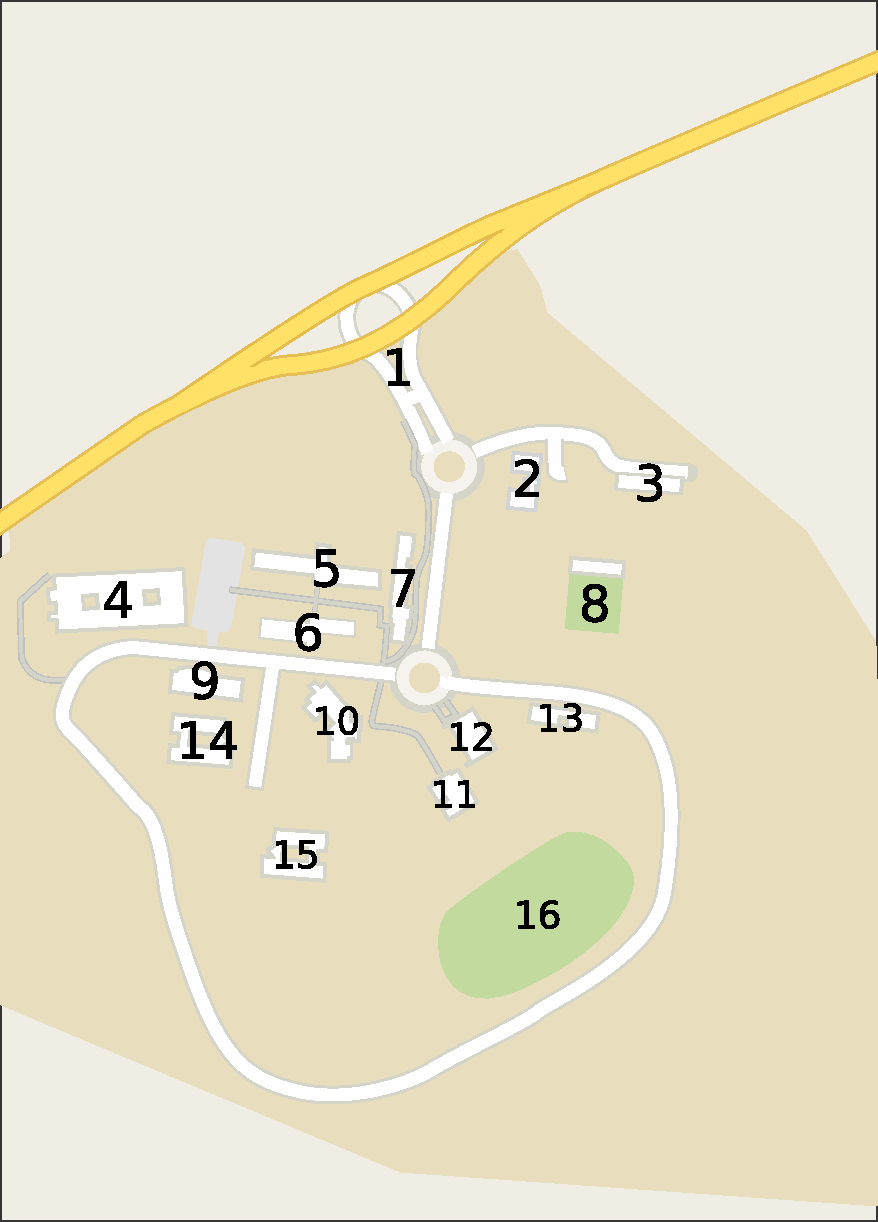
\includegraphics[width=0.85\textwidth]{image.pdf}
  \caption{\\1. Portaria 2. Administração 3. Almoxarifado\\4. ATLab (Prédio Roxo) 5. Laboratórios 6. AT (Aulas Teóricas)\\7. DiGRA 8. Quadra 9. AT-2 (Prédio Vermelho)\\10. Biblioteca 11. Área de Vivência 12. Restaurante Universitário\\13. Ambulatório 14. CCGT (Prédio Verde) 15. CCTS (Prédio Amarelo)\\16. Pista de corrida/Campo de futebol}
\end{figure}

\thispagestyle{empty}

\end{document}
